correlated time-series data is equally consistent with each of these
three causal hypotheses, providing the experimentalist with no
inferential power. Experimentally manipulating \(x\) and observing the
output of \(y\), however, allows the scientist to begin to establish
which causal interaction pattern is at work. Consistent with intuition
from neuroscience literature, a rich theoretical literature has
described the central role of interventions in inferring causal
structure from data .

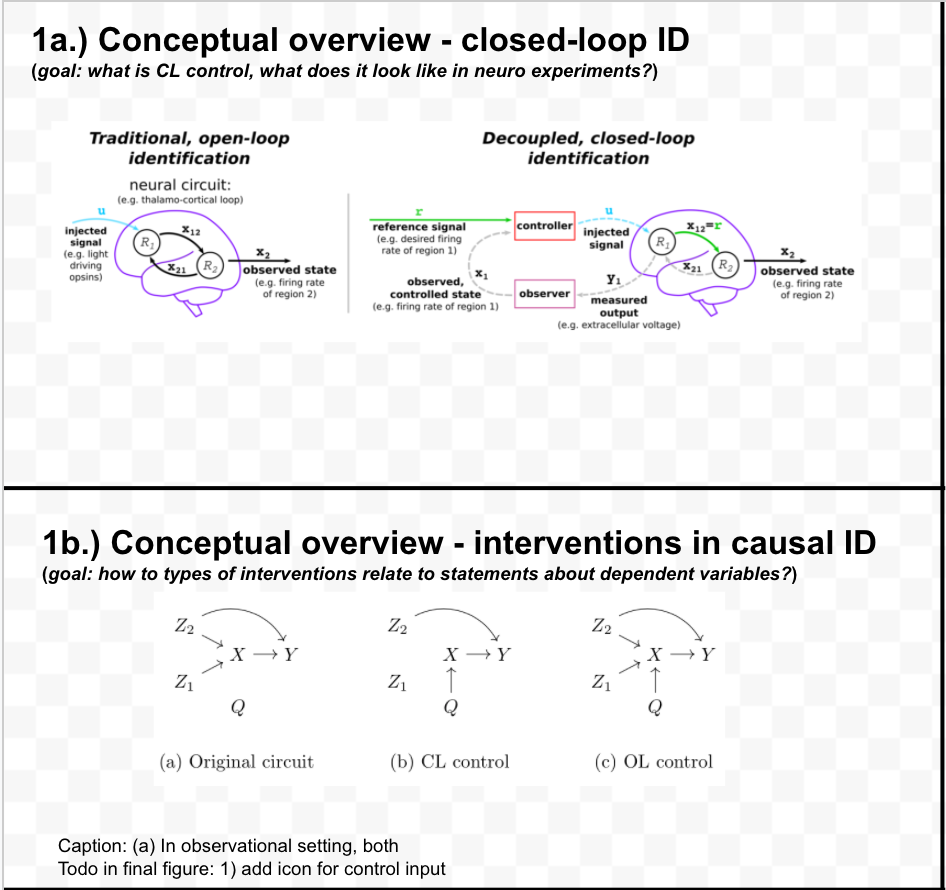
\includegraphics{_annex/clinc/__jpg_figures/core_figure_sketches/figure1_sketch.png}
\textgreater{} \textbf{Figure INTRO:} Examples of the roles
interventions have played in neuroscience. (A) \emph{Passive
observation} does not involve stimulating the brain. In this example,
passive observational data is used to identify patients suffering from
absence seizures. (B) \emph{Open-loop stimulation} involves recording
activity in the brain after perturbing a region with a known input
signal. Using systematic \emph{open-loop stimulation experiments},
Penfield uncovered the spatial organization of h